\chapter{Algunas herramientas de seguridad}
\section{Introducci\'on}
>Por qu\'e utilizar herramientas de seguridad en los sistemas Unix? Ning\'un
sistema operativo se puede considerar `seguro' tal y como se instala por 
defecto\footnote{<Algunos no pueden considerarse `seguros' nunca!}; 
normalmente, cualquier distribuci\'on de un sistema se instala pensando en
proporcionar los m\'{\i}nimos problemas a un administrador que desee poner
la m\'aquina a trabajar inmediatamente, sin tener que preocuparse de la 
seguridad. Es una cuesti\'on de puro {\it marketing}: imaginemos un sistema
Unix que por defecto se instalara en su modo m\'as restrictivo en cuanto a
seguridad; cuando el administrador desee ponerlo en funcionamiento 
conect\'andolo a una red, ofreciendo ciertos servicios, gestionando usuarios y 
perif\'ericos\ldots deber\'a conocer muy bien al sistema, ya que ha de dar
expl\'{\i}citamente los permisos necesarios para realizar cada tarea, con la 
consiguiente p\'erdida de tiempo. Es mucho m\'as productivo para cualquier
empresa desarrolladora de sistemas proporcionarlos completamente abiertos, de 
forma que el administrador no tenga que preocuparse mucho de c\'omo funciona 
cada parte del sistema que acaba de instalar: simplemente inserta el CDROM 
original, el {\it software} se instala, y todo funciona a la primera, 
aparentemente sin problemas\ldots\\
\\Esta pol\'{\i}tica, que lamentablemente siguen casi todas las empresas 
desarrolladoras, convierte a un sistema Unix que no se haya configurado 
m\'{\i}nimamente en un f\'acil objetivo para cualquier atacante. Es m\'as, la
complejidad de Unix hace que un administrador que para aumentar la seguridad de 
su sistema se limite a cerrar ciertos servicios de red o detener algunos
demonios obtenga una sensaci\'on de falsa seguridad: esta persona va a pensar
que su sistema es seguro simplemente por realizar un par de modificaciones en
\'el, cosa que es completamente falsa.
\section{Titan}
Para corroborar la inseguridad de los sistemas Unix instalados tal y como se
distribuyen, o m\'{\i}\-ni\-ma\-men\-te configurados, hemos hecho la prueba con uno de
los sistemas considerados m\'as seguros: Solaris, de la empresa {\it Sun
Microsystems, Inc.}. Hemos instalado Solaris 7 sobre un PC, cerrado la 
mayor\'{\i}a de servicios ofrecidos (en {\tt /etc/inetd.conf}), y controlado el
acceso a otros ({\tt telnet}, {\tt finger}, {\tt ftp}\ldots) mediante 
{\it TCP Wrappers}: justo lo que la mayor parte de administradores har\'{\i}an
antes de poner el sistema a funcionar. Tras estos pasos, hemos ejecutado el
programa de auditor\'{\i}a autom\'atica {\it Titan}, que detecta problemas de
seguridad en la m\'aquina local (para m\'as informaci\'on sobre este {\it 
software} se puede consultar \cite{kn:tit98}).
\subsubsection{Instalaci\'on de {\it Titan}}
Hemos elegido {\it Titan} justamente por ser uno de los programas m\'as 
f\'acilmente instalables sobre SunOS o Solaris: al tratarse de un conjunto de
{\it shellscripts}, el administrador no ha de preocuparse por ning\'un proceso
de compilaci\'on (con los posibles errores que \'este puede causar), ni 
conocer t\'ecnicas avanzadas de seguridad para poder utilizarlo (como otros
programas que presentan una multitud de opciones diferentes que se pueden 
combinar entre ellas, de forma que quien los quiera utilizar debe conocer 
bastante bien ciertos t\'erminos de Unix y de la seguridad, que no suelen ser
triviales). Tanto la instalaci\'on de {\it Titan} como su ejecuci\'on son 
muy sencillos.\\
\\Para instalar {\it Titan}, una vez desempaquetado el fichero, hemos de 
ejecutar simplemente\\{\tt Titan-Config}, con la opci\'on {\tt -i} (la opci\'on 
{\tt -d} desinstala el {\it software}. El programa de instalaci\'on nos 
preguntar\'a si deseamos hacer copias de seguridad de los ficheros que se
modifiquen al ejecutar {\it Titan}; por nuestra seguridad, podemos decirle que
s\'{\i} ({\tt y}):
\begin{verbatim}
anita:/export/home/toni/Security/Tools# gzip -d Titan,v3.0.FCS.tar.gz
anita:/export/home/toni/Security/Tools# tar xvf Titan,v3.0.FCS.tar
anita:/export/home/toni/Security/Tools# cd Titan,v3.0.FCS
anita:/export/home/toni/Security/Tools/Titan,v3.0.FCS# ./Titan-Config -i
checking for dependencies...
finding out where we are...
we are in '/export/home/toni/Security/Tools/Titan,v3.0.FCS'

checking out your system...
this system runs: SunOS-5.7-i86pc
we will be using: sol2x86

setting up links...
removing old links...
linking bin into path...
linking lib into path...
linking logs into path...
linking src into path...
linking tmp into path...
linking done.
cleaning up is_root, sanity_check, Titan...
pulling in local Titan script...
 
Run Titan utilites with 'Titan -[v,f,i]' after reading the Docs...
			OR
Run Titan using a config file. (Titan -c sample.Server) after reading the Docs  
 
Titan can backup all of the files it modifies; This is recommended
proceed? y/n: y
Okay... Checking for backup program...
Found backtit.sh - Backing up system files now... This might take a while..
Creating backup dir in : /export/home/toni/Security/Tools/Titan,v3.0.FCS/\
     arch/sol2sun4/bin/Backup//1013990418
Generating listings.....
Calculating and backing up files now...................................\
     ............ Done!!
...
...
Saved off 44 files to: /export/home/toni/Security/Tools/Titan,v3.0.FCS/\
     arch/sol2sun4/bin/Backup//1013990418
See details in savelist: /export/home/toni/Security/Tools/Titan,v3.0.FCS/\
     arch/sol2sun4/bin/Backup//1013990418/../SaveList.1013990418
Restore by running /export/home/toni/Security/Tools/Titan,v3.0.FCS/\
     arch/sol2sun4/bin/lib/untit.sh -[g,r]
anita:/export/home/toni/Security/Tools/Titan,v3.0.FCS# 
\end{verbatim}
Una vez instalado {\it Titan} (todo a partir del directorio actual, no genera
ficheros en ning\'un otro lugar de nuestros sistemas de archivos) podemos
ejecutar ya el programa de auditor\'{\i}a, con la opci\'on {\tt -v} para que no
realice ning\'un cambio en nuestro sistema, sino que simplemente se limite a
informarnos de los posibles problemas de seguridad que podemos tener; si 
deseamos ver el funcionamiento de cada uno de los {\it shellscripts} invocados
por {\it Titan}, podemos utilizar la opci\'on {\tt -i}, y si lo que queremos
es solucionar los problemas detectados, la opci\'on {\tt -f} (cuidado si 
hacemos esto, la pol\'{\i}tica de seguridad de {\it Titan} es tan estricta que
podemos dejar al sistema s\'olamente utilizable por el {\it root}).
\subsubsection{Ejecuci\'on de {\it Titan}}
En nuestro caso, queremos que {\it Titan} nos informe de los problemas de
seguridad que detecte, pero que no los solucione \'el:
\begin{verbatim}
anita:/export/home/toni/Security/Tools/Titan,v3.0.FCS# ./Titan -v

_____________________________________________________
*=*=*=*=* Running modules/add-umask.sh now.....
Output to ../logs/modules/add-umask.sh.V.042506
-----------------------------------------------------
No umask file /etc/init.d/umask.sh found

_____________________________________________________
*=*=*=*=* Running modules/adjust-arp-timers.sh now.....
Output to ../logs/modules/adjust-arp-timers.sh.V.042506
-----------------------------------------------------

Checking for ARP timers in /etc/rc2.d/S69inet

ARP timers are not set - FAILS CHECK


_____________________________________________________
*=*=*=*=* Running modules/adjust.syn-timeout.sh now.....
Output to ../logs/modules/adjust.syn-timeout.sh.V.042506
-----------------------------------------------------
ERROR - This script is Only needed on Solaris 2.4 and older
please see Sun's patch (Patch 103582-11 currently) for a better fix

_____________________________________________________
*=*=*=*=* Running modules/automount.sh now.....
Output to ../logs/modules/automount.sh.V.042506
-----------------------------------------------------
File /etc/rc2.d/S74autofs exists...
Automounter =
/usr/lib/autofs/automountd /usr/sbin/automount /usr/bin/pkill - FAILS CHECK

_____________________________________________________
*=*=*=*=* Running modules/create-issue.sh now.....
Output to ../logs/modules/create-issue.sh.V.042506
-----------------------------------------------------
Cannot read /etc/issue - FAILS CHECK

_____________________________________________________
*=*=*=*=* Running modules/decode.sh now.....
Output to ../logs/modules/decode.sh.V.042506
-----------------------------------------------------
Decode disabled - PASSES CHECK

_____________________________________________________
*=*=*=*=* Running modules/disable-L1-A.sh now.....
Output to ../logs/modules/disable-L1-A.sh.V.042506
-----------------------------------------------------
./modules/disable-L1-A.sh: ./sanity_check: No such file or directory

_____________________________________________________
*=*=*=*=* Running modules/disable-NFS.bind.sh now.....
Output to ../logs/modules/disable-NFS.bind.sh.V.042506
-----------------------------------------------------
Verifying port settings using ndd
privileged port definition is currently set to 1024

You should run disable-NFS.bind.sh with the -F option (port=1024)


_____________________________________________________
*=*=*=*=* Running modules/disable-accounts.sh now.....
Output to ../logs/modules/disable-accounts.sh.V.042506
-----------------------------------------------------
Checking 11 Users....
Checking that shell set to noshell for:
daemon bin adm lp uucp nuucp listen nobody noaccess nobody4 ppp
Verify shell status....

daemon shell = - FAILS CHECK
bin shell = - FAILS CHECK
adm shell = - FAILS CHECK
lp shell = - FAILS CHECK
uucp shell = - FAILS CHECK
nuucp shell = /usr/lib/uucp/uucico - FAILS CHECK
listen shell = - FAILS CHECK
nobody shell = - FAILS CHECK
noaccess shell = - FAILS CHECK
nobody4 shell = - FAILS CHECK
ppp shell = /usr/sbin/pppls - FAILS CHECK

11 Users Not Secured Out Of 11

_____________________________________________________
*=*=*=*=* Running modules/disable-core.sh now.....
Output to ../logs/modules/disable-core.sh.V.042506
-----------------------------------------------------
Core dump size has not been set: FAILS CHECK

_____________________________________________________
*=*=*=*=* Running modules/disable-ping-echo.sh now.....
Output to ../logs/modules/disable-ping-echo.sh.V.042506
-----------------------------------------------------
Ping echo response allowed - FAILED CHECK
Run ./modules/disable-ping-echo.sh with -[Ff] to fix...


_____________________________________________________
*=*=*=*=* Running modules/disable_ip_holes.sh now.....
Output to ../logs/modules/disable_ip_holes.sh.V.042506
-----------------------------------------------------
Checking ip_forwarding...
ip_forwarding disabled - PASSES CHECK
Checking ip_forward_src_routed...
ip_forward_src_routed disabled - PASSES CHECK
Checking ip_forward_directed_broadcasts...
ip_forward_directed_broadcasts disabled - PASSES CHECK
Checking ip_ignore_redirect...
ip_ignore_redirect enabled - PASSES CHECK
Checking ip_strict_dst_multihoming...
ip_strict_dst_multihoming enabled - PASSES CHECK
System configured as 'notrouter' - PASSES CHECK

_____________________________________________________
*=*=*=*=* Running modules/dmi-2.6.sh now.....
Output to ../logs/modules/dmi-2.6.sh.V.042506
-----------------------------------------------------
ERROR - This script is Only supported on Solaris 2.6 and newer, 
please use one of the other scripts for your OS

_____________________________________________________
*=*=*=*=* Running modules/eeprom.sh now.....
Output to ../logs/modules/eeprom.sh.V.042506
-----------------------------------------------------
Architecture = i86pc
Eeprom security-mode not supported on this host

_____________________________________________________
*=*=*=*=* Running modules/file-own.sh now.....
Output to ../logs/modules/file-own.sh.V.042506
-----------------------------------------------------
Checking /usr file ownership
Found 25345 files in /usr that should be root owned
Checking /sbin file ownership
Found 13 files in /sbin that should be root owned
Checking /usr group permissions
Found 0 files in /usr that should be set group g-w
Checking /sbin group permissions
Found 0 files in /sbin that should be set group g-w
Checking /etc group permissions
Found 0 files in /etc that should be set group g-w
Checking /opt group permissions
Found 0 files in /opt that should be set group g-w

_____________________________________________________
*=*=*=*=* Running modules/fix-cronpath.sh now.....
Output to ../logs/modules/fix-cronpath.sh.V.042506
-----------------------------------------------------
File /var/spool/cron/crontabs/root exists; continuing
       /etc is not writable by world - PASSES CHECK.
       /etc is not writeable by group - PASSES CHECK.
       /etc/cron.d is not writable by world - PASSES CHECK.
       /etc/cron.d is not writeable by group - PASSES CHECK.
       /usr is not writable by world - PASSES CHECK.
drwxrwxr-x  32 root         1024 Oct  8 00:58 /usr
       /usr is writeable by group - FAILS CHECK
       /usr/sbin is not writable by world - PASSES CHECK.
drwxrwxr-x   5 root         4608 Sep 24 01:32 /usr/sbin
       /usr/sbin is writeable by group - FAILS CHECK
       /usr/lib is not writable by world - PASSES CHECK.
drwxrwxr-x  42 root        10240 Oct  8 00:55 /usr/lib
       /usr/lib is writeable by group - FAILS CHECK
       /usr/lib/fs is not writable by world - PASSES CHECK.
drwxrwxr-x  13 root          512 Sep 23 18:33 /usr/lib/fs
       /usr/lib/fs is writeable by group - FAILS CHECK
       /usr/lib/fs/nfs is not writable by world - PASSES CHECK.
       /usr/lib/fs/nfs is not writeable by group - PASSES CHECK.
       /usr/bin is not writable by world - PASSES CHECK.
drwxrwxr-x   3 root         7680 Oct  8 00:52 /usr/bin
       /usr/bin is writeable by group - FAILS CHECK
    
    /etc/cron.d/logchecker ownership should be changed to root 
    /usr/lib/newsyslog ownership should be changed to root 
    /usr/bin/rdate ownership should be changed to root 
    /usr/sbin/rtc ownership should be changed to root 
    
         No cron.allow file - FAILS CHECK

_____________________________________________________
*=*=*=*=* Running modules/fix-modes.sh now.....
Output to ../logs/modules/fix-modes.sh.V.042506
-----------------------------------------------------
Only supported on Solaris 2.2 thru 2.6

_____________________________________________________
*=*=*=*=* Running modules/fix-stack.sh now.....
Output to ../logs/modules/fix-stack.sh.V.042506
-----------------------------------------------------
ERROR - This script is Only known to work on Solaris 2.5.[0-5]

_____________________________________________________
*=*=*=*=* Running modules/fix-stack.sol2.6.sh now.....
Output to ../logs/modules/fix-stack.sol2.6.sh.V.042506
-----------------------------------------------------
Stack Protection not currently set - Run fix-stack.sol2.6.sh -F

_____________________________________________________
*=*=*=*=* Running modules/ftpusers.sh now.....
Output to ../logs/modules/ftpusers.sh.V.042506
-----------------------------------------------------
No /etc/ftpusers file in place...
Should contain at least:

root
daemon
sys
bin
adm
lp
smtp
uucp
nuucp
listen
nobody
noaccess
news
ingres
audit
admin
sync
nobody4

Please Run with '-F/f' to Fix - FAILS CHECK

_____________________________________________________
*=*=*=*=* Running modules/hosts.equiv.sh now.....
Output to ../logs/modules/hosts.equiv.sh.V.042506
-----------------------------------------------------
No /etc/hosts.equiv - PASSES CHECK

_____________________________________________________
*=*=*=*=* Running modules/inetd.sh now.....
Output to ../logs/modules/inetd.sh.V.042506
-----------------------------------------------------
File /etc/inet/inetd.conf exists - Checking...
name Closed - PASSES CHECK
exec Closed - PASSES CHECK
comsat Closed - PASSES CHECK
talk Open - FAILS CHECK
uucp Closed - PASSES CHECK
smtp Closed - PASSES CHECK
tftp Closed - PASSES CHECK
finger Open - FAILS CHECK
systat Closed - PASSES CHECK
netstat Closed - PASSES CHECK
rquotad Closed - PASSES CHECK
rusersd Closed - PASSES CHECK
sprayd Closed - PASSES CHECK
walld Closed - PASSES CHECK
rexd Closed - PASSES CHECK
shell Closed - PASSES CHECK
login Closed - PASSES CHECK
exec Closed - PASSES CHECK
comsat Closed - PASSES CHECK
time Closed - PASSES CHECK
echo Closed - PASSES CHECK
discard Closed - PASSES CHECK
daytime Closed - PASSES CHECK
chargen Closed - PASSES CHECK
100087 Closed - PASSES CHECK
rwalld Closed - PASSES CHECK
rstatd Closed - PASSES CHECK
100068 Closed - PASSES CHECK
100083 Closed - PASSES CHECK
100221 Closed - PASSES CHECK
fs Closed - PASSES CHECK
ufsd Closed - PASSES CHECK
100232 Closed - PASSES CHECK
100235 Closed - PASSES CHECK
536870916 Closed - PASSES CHECK

_____________________________________________________
*=*=*=*=* Running modules/keyserv.sh now.....
Output to ../logs/modules/keyserv.sh.V.042506
-----------------------------------------------------
In /etc/rc2.d/S71rpc keyserv ; user nobody enabled - FAILS CHECK

_____________________________________________________
*=*=*=*=* Running modules/log-tcp.sh now.....
Output to ../logs/modules/log-tcp.sh.V.042506
-----------------------------------------------------

_____________________________________________________
*=*=*=*=* Running modules/loginlog.sh now.....
Output to ../logs/modules/loginlog.sh.V.042506
-----------------------------------------------------
No /var/adm/loginlog file - FAILS CHECK

_____________________________________________________
*=*=*=*=* Running modules/lpsched.sh now.....
Output to ../logs/modules/lpsched.sh.V.042506
-----------------------------------------------------
In /etc/rc2.d/S80lp lpsched is enabled - FAILS CHECK

_____________________________________________________
*=*=*=*=* Running modules/nfs-portmon.sh now.....
Output to ../logs/modules/nfs-portmon.sh.V.042506
-----------------------------------------------------
NFS port monitor disabled - FAILS CHECK

_____________________________________________________
*=*=*=*=* Running modules/nsswitch.sh now.....
Output to ../logs/modules/nsswitch.sh.V.042506
-----------------------------------------------------
passwd -> files - PASSES CHECK
group -> files - PASSES CHECK
hosts -> files - PASSES CHECK
networks -> files - PASSES CHECK
protocols -> files - PASSES CHECK
rpc -> files - PASSES CHECK
ethers -> files - PASSES CHECK
netmasks -> files - PASSES CHECK
bootparams -> files - PASSES CHECK
publickey -> files - PASSES CHECK
netgroup -> files - PASSES CHECK
automount -> files - PASSES CHECK
aliases -> files - PASSES CHECK
services -> files - PASSES CHECK
sendmailvars -> files - PASSES CHECK
15 of 15 entries set to files as default - PASSES CHECK

_____________________________________________________
*=*=*=*=* Running modules/nuke-sendmail.sh now.....
Output to ../logs/modules/nuke-sendmail.sh.V.042506
-----------------------------------------------------
Sendmail is enabled in /etc/rc2.d/S88sendmail - FAILS CHECK

_____________________________________________________
*=*=*=*=* Running modules/pam-rhosts-2.6.sh now.....
Output to ../logs/modules/pam-rhosts-2.6.sh.V.042506
-----------------------------------------------------
PAM allows rhosts for rlogin : FAILS CHECK
PAM allows rhosts for rsh : FAILS CHECK

_____________________________________________________
*=*=*=*=* Running modules/passwd.sh now.....
Output to ../logs/modules/passwd.sh.V.042506
-----------------------------------------------------
All accounts have passwords - PASSES CHECK

_____________________________________________________
*=*=*=*=* Running modules/powerd.sh now.....
Output to ../logs/modules/powerd.sh.V.042506
-----------------------------------------------------
Power management not set to be run by root - FAILS CHECK

_____________________________________________________
*=*=*=*=* Running modules/psfix.sh now.....
Output to ../logs/modules/psfix.sh.V.042506
-----------------------------------------------------
Could not find /etc/rc3.d/S79tmpfix - FAILS CHECK
Run with -[Ff] option to fix

_____________________________________________________
*=*=*=*=* Running modules/rhosts.sh now.....
Output to ../logs/modules/rhosts.sh.V.042506
-----------------------------------------------------
Running against /etc/passwd...

_____________________________________________________
*=*=*=*=* Running modules/rootchk.sh now.....
Output to ../logs/modules/rootchk.sh.V.042506
-----------------------------------------------------
        /.login - Clean of . - PASSES CHECK
        /etc/.login - Clean of . - PASSES CHECK
        /etc/default/login - Clean of . - PASSES CHECK
        /.cshrc - Clean of . - PASSES CHECK
       /etc/skel/local.cshrc - Contains . - FAILS CHECK
set path=(/bin /usr/bin /usr/ucb /etc .)
        /etc/skel/local.login - Clean of . - PASSES CHECK
        /etc/skel/local.profile - Clean of . - PASSES CHECK
        /.profile - Clean of . - PASSES CHECK
        /etc/profile - Clean of . - PASSES CHECK

_____________________________________________________
*=*=*=*=* Running modules/routed.sh now.....
Output to ../logs/modules/routed.sh.V.042506
-----------------------------------------------------

The route daemon advertises routes - FAILS CHECK

_____________________________________________________
*=*=*=*=* Running modules/sendmail.sh now.....
Output to ../logs/modules/sendmail.sh.V.042506
-----------------------------------------------------
No sendmail.cf.titan2 exists - FAILS CHECK
Run with -[Ff] option to fix.
Checking for smrsh
smrsh not found in /sbin - FAILS CHECK

_____________________________________________________
*=*=*=*=* Running modules/smtp-banner.sh now.....
Output to ../logs/modules/smtp-banner.sh.V.042506
-----------------------------------------------------
No /etc/mail/sendmail.cf exists - FAILS CHECK

_____________________________________________________
*=*=*=*=* Running modules/smtpbanner-8.8.sh now.....
Output to ../logs/modules/smtpbanner-8.8.sh.V.042506
-----------------------------------------------------
ERROR - This script is Only supported on patched Solaris 2.6 and newer, 
please use one of the other scripts for your OS

_____________________________________________________
*=*=*=*=* Running modules/snmpdx-2.6.sh now.....
Output to ../logs/modules/snmpdx-2.6.sh.V.042506
-----------------------------------------------------
ERROR - This script is Only supported on Solaris 2.6 and newer, 
please use one of the other scripts for your OS

_____________________________________________________
*=*=*=*=* Running modules/syslog.sh now.....
Output to ../logs/modules/syslog.sh.V.042506
-----------------------------------------------------
File /etc/syslog.conf exists checking contents....
Syslog auth notice messages disabled - FAILS CHECK

_____________________________________________________
*=*=*=*=* Running modules/tcp-sequence.sh now.....
Output to ../logs/modules/tcp-sequence.sh.V.042506
-----------------------------------------------------
TCP_STRONG_ISS=1
/etc/default/inetinit - has the system default . - FAILS CHECK

_____________________________________________________
*=*=*=*=* Running modules/userumask.sh now.....
Output to ../logs/modules/userumask.sh.V.042506
-----------------------------------------------------
 Checking for umask 022 in   
 /etc/.login
 /etc/default/login
 /etc/profile
 /etc/skel/local.cshrc
 /etc/skel/local.login
 /etc/skel/local.profile

       Umask value other than 022 in /etc/.login - FAILS CHECK
       Umask value other than 022 in /etc/.login - FAILS CHECK
       Umask value 022 in /etc/profile - PASSES CHECK
       Umask value 022 in /etc/skel/local.cshrc - PASSES CHECK
       Umask value other than 022 in /etc/skel/local.login - FAILS CHECK
       Umask value other than 022 in /etc/skel/local.profile - FAILS CHECK

       UMASK value 022 in /etc/default/login - PASSES CHECK

_____________________________________________________
*=*=*=*=* Running modules/utmp.sh now.....
Output to ../logs/modules/utmp.sh.V.042506
-----------------------------------------------------
File utmp permissions o-w - PASSES CHECK
File utmp permissions o-w - PASSES CHECK


_____________________________________________________
*=*=*=*=* Running modules/vold.sh now.....
Output to ../logs/modules/vold.sh.V.042506
-----------------------------------------------------

File /etc/rc2.d/S92volmgt and /usr/sbin/vold exists - FAILS CHECK

Run with -[Ff] option to fix

_____________________________________________________
*=*=*=*=* Running modules/ziplock.sh now.....
Output to ../logs/modules/ziplock.sh.V.042506
-----------------------------------------------------

Unfortunately this is a FIX ONLY utility.....
As noted in the Introduction statement it may break functionality
for all non-root users if run -F

The list of files is as follows and may be manually modified
by editing this script and inserting/commenting out as you
like. Just make sure you know what it is you are changing:

The list of binaries that would be modified is:

/usr/bin/at
/usr/kvm/eeprom
/sbin/su
/usr/bin/atq
/usr/bin/atrm
/usr/bin/chkey
/usr/bin/crontab
/usr/bin/eject
/usr/bin/fdformat
/usr/bin/newgrp
/usr/bin/ps
/usr/bin/rcp
/usr/bin/rdist
/usr/bin/rlogin
/sbin/sulogin
/usr/bin/login
/usr/bin/rsh
/usr/bin/su
/usr/bin/tip
/usr/bin/uptime
/usr/bin/yppasswd
/usr/bin/w
/usr/bin/ct
/usr/bin/cu
/usr/bin/uucp
/usr/bin/uuglist
/usr/bin/uuname
/usr/bin/uustat
/usr/bin/uux
/usr/lib/exrecover
/usr/lib/fs/ufs/ufsdump
/usr/lib/fs/ufs/ufsrestore
/usr/lib/pt_chmod
/usr/lib/sendmail.mx
/usr/lib/acct/accton
/usr/sbin/allocate
/usr/sbin/mkdevalloc
/usr/sbin/mkdevmaps
/usr/sbin/ping
/usr/sbin/sacadm
/usr/sbin/static/rcp
/usr/sbin/whodo
/usr/sbin/deallocate
/usr/sbin/list_devices
/usr/openwin/bin/xlock
/usr/openwin/bin/xdm
/usr/openwin/lib/mkcookie
/usr/ucb/ps
/usr/vmsys/bin/chkperm
/usr/bin/passwd
/usr/bin/csh
/etc/lp/alerts/printer
/usr/kvm/crash
/usr/kvm/eeprom
/usr/bin/netstat
/usr/bin/nfsstat
/usr/bin/write
/usr/bin/ipcs
/usr/sbin/arp
/usr/sbin/prtconf
/usr/sbin/swap
/usr/sbin/sysdef
/usr/sbin/wall
/usr/sbin/dmesg
/usr/openwin/bin/Xsun
/usr/openwin/bin/wsinfo
/usr/openwin/bin/mailtool
/usr/openwin/bin/xload
/usr/openwin/bin/kcms_calibrate
/usr/openwin/bin/kcms_configure
/usr/openwin/bin/kcms_server
/var/adm/messages
/var/log/syslog
/var/adm/pacct
anita:/export/home/toni/Security/Tools/Titan,v3.0.FCS#
\end{verbatim}
Mirando por encima el resultado ofrecido por {\it Titan}, vemos que ha 
detectado {\bf <casi 50 posibles problemas!} (cada mensaje {\sc FAILS CHECK} 
denota una alarma, mientras que cada mensaje {\sc PASSES CHECK} denota un 
test satisfactorio).\\
\\A la vista de estos resultados, y teniendo en cuenta que hemos utilizado una
versi\'on m\'as o menos moderna de Solaris (la versi\'on 7 10/98, si 
hubi\'eramos comprobado una versi\'on de Solaris o SunOS m\'as antigua 
habr\'{\i}amos detectado seguramente muchos m\'as problemas), parece claro que
un sistema Unix instalado tal y como se distribuye, o con una configuraci\'on
de seguridad m\'{\i}nima --nuestro caso--, representa un grave problema ya no
s\'olo para la m\'aquina en cuesti\'on, sino para toda la red en la que 
trabaja. Por tanto, el uso de cualquier herramienta que nos ayude a solucionar,
o al menos a localizar problemas, va a ser \'util.
\section{TCP Wrappers}
En el punto \ref{serv} habl\'abamos de los servicios ofrecidos desde nuestra 
m\'aquina; all\'{\i} comentamos que cualquiera de ellos es una potencial puerta 
de entrada para un atacante, por lo que es muy recomendable cerrar todos los
que no necesitemos; vimos un esquema todo o nada: u ofrec\'{\i}amos un servicio
a toda la red o lo deneg\'abamos, pero no hab\'{\i}a t\'ermino medio.\\
\\Hay una serie de servicios como {\it telnet} o {\it ftp} que habitualmente no 
vamos a poder cerrar, ya que los usuarios necesitar\'an conectar al servidor 
para trabajar en \'el o para transferir ficheros; en estos casos es peligroso 
permitir que cualquier m\'aquina de Internet tenga la posibilidad de acceder
a nuestros recursos, por lo que se suele utilizar un programa denominado 
{\it TCP Wrappers} (\cite{kn:ven92}) para definir una serie de redes o 
m\'aquinas autorizados a
conectar con nosotros. Aqu\'{\i} veremos como instalar este {\it software} 
-- en su versi\'on 7.6 -- y su configuraci\'on b\'asica para que no todo el 
mundo pueda contactar con nosotros. Actualmente, cualquier administrador que 
desee un m\'{\i}nimo de seguridad ha de instalar {\it TCP Wrappers} en sus
equipos; incluso algunos Unices como Linux o BSDI lo ofrecen por defecto al 
instalar el operativo. Cabe decir que la configuraci\'on del programa puede
ser muy elaborada y con muchas opciones; aqu\'{\i} veremos la forma m\'as 
b\'asica, que suele ser autom\'atica mediante {\tt make install}
\footnote{Aqu\'{\i} explicamos el proceso `a mano' simplemente para entender 
c\'omo funciona.}. 
Para configuraciones m\'as avanzadas se recomienda consultar los ficheros de 
ayuda.\\
\\En nuestro caso vamos a instalar {\it TCP Wrappers} sobre una m\'aquina
Silicon Graphics corriendo IRIX 6.2:
\tt
\begin{quote}
\begin{verbatim}
llegona_(/) # uname -a
IRIX64 llegona 6.2 06101031 IP28
llegona_(/) # 
\end{verbatim}
\end{quote}
\rm
No vamos a entrar aqu\'{\i} en como compilar el software (para ello se puede
consultar el fichero {\tt README}); asumiremos que ya lo tenemos compilado y
el resultado est\'a, por ejemplo, en el directorio {\tt /tmp/tcp$\_$wrappers$\_$7.6/}.
Tras compilar el {\it software} se habr\'an generado una serie de ficheros
ejecutables que hemos de copiar a un destino definitivo, por ejemplo a 
{\tt /etc/usr/sbin/}:
\begin{quote}
\begin{verbatim}
llegona_(/tmp/tcp_wrappers_7.6) # cp `find . -type f -perm -700` /usr/sbin/
llegona_(/tmp/tcp_wrappers_7.6) # 
\end{verbatim}
\end{quote}
Una vez en su destino definitivo, hemos de modificar el fichero {\tt 
/etc/inetd.conf} para indicarle a {\tt inetd} que ha de utilizar el demonio 
{\tt tcpd} (la parte m\'as importante de {\it TCP Wrappers}) a la hora de 
servir peticiones; para ello, una entrada de la forma 
\begin{quote}
\begin{verbatim}
telnet  stream  tcp     nowait  root    /usr/etc/telnetd 
\end{verbatim}
\end{quote}
se convertir\'a en una como 
\begin{quote}
\begin{verbatim}
telnet  stream  tcp     nowait  root    /usr/sbin/tcpd  /usr/etc/telnetd 
\end{verbatim}
\end{quote}
Como vemos, en lugar de que {\tt inetd} ejecute directamente el demonio
correspondiente a cada servicio, ejecuta el {\it wrapper}, y es \'este el 
encargado de controlar la ejecuci\'on del demonio real.\\
\\Tras haber modificado convenientemente {\tt /etc/inetd.conf} hemos de
configurar
los servicios que vamos a ofrecer a diferentes m\'aquinas o redes; seguiremos 
una pol\'{\i}tica restrictiva: todo lo no expl\'{\i}citamente permitido, est\'a
negado. Para ello, en el archivo {\tt /etc/hosts.allow} indicamos que servicios
ofrecemos y a d\'onde lo hacemos\footnote{Realmente, tambi\'en es posible
especificar acciones a realizar al recibir una conexi\'on; se puede consultar
la sintaxis exacta en la p\'agina del manual de {\tt hosts$\_$access(5)}.}, de 
la siguiente forma:
\it
\begin{center}
demonio: maquinas
\end{center}
\rm
Donde {\it `demonio'} es el nombre del demonio encargado de atender el servicio
correspondiente \\({\tt sendmail}, {\tt telnetd}, {\tt fingerd}\ldots), y {\it
`maquinas'} es la especificaci\'on de los {\it hosts} a los que les est\'a
permitida la conexi\'on a cada servicio; se trata de una lista separada por 
espacios donde podemos incluir desde nombres de sistemas o direcciones IP hasta
subdominios, pasando por palabras reservadas como {\tt ALL}.
As\'{\i}, si por ejemplo queremos ofrecer todo a las
m\'aquinas {\tt .dsic.upv.es}, {\it telnet} a {\tt andercheran.aiind.upv.es} y
{\tt luisvive.euiti.upv.es}, y 
{\tt ftp} a toda la UPV, tendremos un {\tt /etc/hosts.allow} de la forma
siguiente:
\begin{quote}
\begin{verbatim}
llegona_(/) # cat /etc/hosts.allow
ALL: .dsic.upv.es
telnetd: andercheran.aiind.upv.es luisvive.euiti.upv.es
ftpd: .upv.es
llegona_(/) #
\end{verbatim}
\end{quote}
Acabamos de configurar los sistemas con acceso a ciertos demonios; para indicar
a {\it TCP Wrappers} que nuestros servicios no van a ser ofertados a nadie 
m\'as, creamos el fichero {\tt /etc/hosts.deny} y denegamos todo a todos:
\tt
\begin{quote}
\begin{verbatim}
llegona_(/) # cat /etc/hosts.deny
ALL: ALL
llegona_(/) #
\end{verbatim}
\end{quote}
\rm
Una vez hemos configurado todo, hemos de hacer que {\tt inetd} relea su fichero
de configuraci\'on envi\'andole la se\~nal {\sc sighup}, por ejemplo con
la orden {\tt killall -HUP inetd}\footnote{Concretamente en IRIX este mecanismo
no funciona, hay que matar el demonio y volverlo a lanzar.}. A partir de ese 
momento los cambios han tenido efecto; en funci\'on de nuestro {\tt 
/etc/syslog.conf}, pero generalmente en archivos como {\tt /var/adm/SYSLOG} o
{\tt /var/adm/messages} vamos a poder ver las conexiones aceptadas y las
rehusadas:
\tt
\begin{quote}
\begin{verbatim}
Dec 2 02:16:47 llegona ftpd[18234]: refused connect from bill.microsoft.com
Dec 2 02:45:23 llegona telnetd[18234]: connect from corbella.dsic.upv.es
\end{verbatim}
\end{quote}
\rm
Cuando alguien desde una m\'aquina que tiene permiso para acceder a cierto
servicio conecte a \'el no notar\'a nada raro, pero si lo hace desde un equipo
no autorizado, la conexi\'on se cerrar\'a:
\tt
\begin{quote}
\begin{verbatim}
anita:~# telnet llegona.dsic.upv.es
Trying 158.42.49.37...
Connected to llegona.dsic.upv.es
Escape character is '^]'.
llegona login: Connection closed by foreign host.
anita:~# 
\end{verbatim}
\end{quote}
\rm
\section{SSH}
Tradicionalmente el intercambio de datos entre sistemas Unix (desde la 
transferencia de ficheros o la compartici\'on de archivos v\'{\i}a NFS hasta el
acceso remoto) se ha realizado utilizando mecanismos en los que la seguridad 
era un factor poco importante frente a otros como la velocidad o la 
disponibilidad. Sin embargo, conforme ha ido aumentando 
la calidad de los medios de transmisi\'on (en la actualidad cualquier peque\~na
organizaci\'on tiene al menos una red {\it Fast Ethernet} capaz de alcanzar 
velocidades de 100 Mbps, cuando no una ATM, una FDDI o incluso una GigaEthernet
que alcanza los 1000 Mbps de velocidad), y tambi\'en conforme ha ido aumentando
la peligrosidad de las redes, especialmente de Internet, se ha ido considerando
m\'as el grave problema que implica una transmisi\'on de datos en texto claro,
ya sea un {\it telnet}, un {\it ftp} o incluso la transmisi\'on de datos que
tiene lugar al utilizar sistemas de ficheros en red. Por suerte, en la 
actualidad, casi nadie sigue usando los medios cl\'asicos de intercambio de 
datos entre equipos Unix: por ejemplo, muy poca gente sigue conectando mediante 
{\it telnet} a m\'aquinas remotas, mientras que hace unos pocos a\~nos era
habitual ver estas conexiones incluso entre m\'aquinas separadas por multitud
de redes. Casi todos los mecanismos cl\'asicos se han reemplazado por 
protocolos que incorporan el cifrado en mayor o menor medida, de forma que 
un pirata que captura datos transmitidos entre sistemas lo tiene muy 
dif\'{\i}cil para conseguir informaci\'on importante, como una clave de 
usuario; ejemplos de protocolos que incorporan la criptograf\'{\i}a son SSL 
({\it Secure Socket Layer}) o TCFS ({\it Transparent Cryptographic File 
System}, del que ya hemos hablado en este proyecto).\\
\\Dentro de todo estos modelos considerados seguros est\'a {\it Secure Shell} 
({\sc ssh}), un {\it software} cuya principal funci\'on es permitir la 
conexi\'on remota segura a sistemas a trav\'es de canales inseguros, aunque 
tambi\'en se utiliza para la ejecuci\'on de \'ordenes en ese sistema remoto o 
transferir ficheros desde o hacia \'el de manera fiable (\cite{kn:ylo96}); es, 
por tanto, el 
sustituto ideal de \'ordenes como {\tt telnet}, {\tt ftp} o {\tt r$\ast$} de 
Unix BSD. Todo esto utilizando RSA, SecurID, Kerberos, TIS o la autenticaci\'on 
cl\'asica de Unix ({\it login} y {\it password}). Adem\'as, y entre otras 
caracter\'{\i}sticas, {\sc ssh} tambi\'en soporta el cifrado autom\'atico 
en sesiones X-Window o modelos de seguridad m\'as avanzados, como el cifrado en
NFS o la construcci\'on de redes privadas virtuales; su c\'odigo fuente es
libre para uso no comercial (existe otro {\it software} casi completamente 
compatible con {\tt ssh} y completamente libre, denominado {\it OpenSSH}) y se 
puede obtener en {\tt http://www.ssh.fi/}. En la actualidad, {\sc
ssh} funciona sobre la mayor\'{\i}a de clones de Unix (tambi\'en existen 
versiones para Windows y MacOS), y es ampliamente utilizado en todo tipo de 
entornos, desde universidades a bancos pasando por empresas de cualquier 
sector.\\
\\{\sc ssh} est\'a formado por un programa servidor, {\tt sshd}, varios 
programas cliente ({\tt ssh} y {\tt scp} principalmente) y peque\~nas 
aplicaciones para su
configuraci\'on, como {\tt ssh-add}, {\tt ssh-keygen} o {\tt ssh-agent}. El 
programa demonio
({\tt sshd}) se ejecuta en la m\'aquina contra la cual conectamos, mientras
que los clientes se han de ejecutar evidentemente en el sistema desde el cual
conectamos; as\'{\i}, podemos iniciar una sesi\'on en la m\'aquina remota con
una orden como la siguiente:
\begin{quote}
\begin{verbatim}
anita:~# ssh -l toni rosita
toni's password: 
Last login: Thu Apr  6 03:58:32 2000 from anita
Linux 2.2.6
"A witty saying proves nothing."
                -- Voltaire

rosita:~$
\end{verbatim}
\end{quote}
El par\'ametro {\tt `-l'} nos permite indicar el nombre de usuario en el
sistema remoto (en caso contrario, se utilizar\'a el mismo nombre que se posee
en la m\'aquina local); {\sc ssh} tambi\'en permite especificar desde 
l\'{\i}nea de comandos una orden a ejecutar en la m\'aquina a la que 
conectamos, de forma que cuando esta orden finalice se cerrar\'a la conexi\'on 
entre ambos sistemas:
\begin{quote}
\begin{verbatim}
anita:~# ssh -l toni luisa w
toni's password:
  3:15am  up 5 days,  1:30,  5 users,  load average: 1.12, 1.04, 1.01
USER     TTY      FROM     LOGIN@   IDLE   JCPU   PCPU  WHAT
root     tty1     -        Sat12am  5days  0.02s  0.02s  bash           
toni     ttyp1    :0.0     Sun 3pm  1:02   0.18s  0.13s  telnet rosita 
toni     ttyp2    :0.0     Sun 4am  2.00s  2.40s  2.04s  vi tools.tex 
toni     ttyp4    anita    Tue 1am  0.00s  1.31s  0.02s  w 
anita:~#
\end{verbatim}
\end{quote}
Como hemos podido ver, {\tt ssh} se utiliza b\'asicamente para iniciar sesiones
o ejecutar comandos en un sistema remoto; el otro programa cliente, {\tt scp},
es utilizado para transferir ficheros entre m\'aquinas, de una forma similar
a {\tt rcp}, lo que por ejemplo permite sustituir el {\it ftp} tradicional por
este mecanismo. Si por ejemplo deseamos copiar todos los ficheros del 
directorio {\tt /export/home/toni/} conectando al sistema remoto bajo el nombre
de usuario {\tt toni} en el directorio {\tt /tmp/} de la m\'aquina local, lo 
podemos conseguir con una orden como esta:
\begin{quote}
\begin{verbatim}
luisa:~# scp -r toni@anita:/export/home/toni/ /tmp/
toni's password:
luisa:~#
\end{verbatim}
\end{quote}
Como podemos ver, estamos indicando el nombre de usuario y el del sistema
remotos separados por {\tt `@'}, y separados a su vez de la ruta origen por
el signo {\tt `:'}.\\ 
\\Pero, >qu\'e es lo que realmente hace cualquiera de estos clientes contra el
servidor {\tt sshd}? Si no indicamos lo contrario con la opci\'on {\tt `-p'}, 
el cliente 
conecta al puerto 22 de la m\'aquina servidora y verifica que esta m\'aquina
es realmente con la que queremos conectar, intercambia las claves de cifrado
entre sistemas (cifradas a su vez, para evitar que un atacante pueda obtener
la informaci\'on) y autentica utilizando {\tt .rhosts} y {\tt /etc/hosts.equiv}
(como los protocolos {\tt r-$\ast$}), RSA o claves de usuario; si todo es 
correcto, el servidor asigna una terminal virtual (generalmente) a la conexi\'on
y lanza un {\it shell} interactivo. Podemos ver con detalle este proceso
utilizando la opci\'on {\tt `-v'} del cliente:
\begin{quote}
\begin{verbatim}
luisa:~# ssh -v -l toni luisa
SSH Version 1.2.21 [i486-unknown-linux], protocol version 1.5.
Standard version.  Does not use RSAREF.
luisa: Reading configuration data /etc/ssh_config
luisa: ssh_connect: getuid 0 geteuid 0 anon 0
luisa: Connecting to luisa [192.168.0.2] port 22.
luisa: Allocated local port 1023.
luisa: Connection established.
luisa: Remote protocol version 1.5, remote software version 1.2.21
luisa: Waiting for server public key.
luisa: Received server public key (768 bits) and host key (1024 bits).
luisa: Host 'luisa' is known and matches the host key.
luisa: Initializing random; seed file /root/.ssh/random_seed
luisa: Encryption type: idea
luisa: Sent encrypted session key.
luisa: Received encrypted confirmation.
luisa: Trying rhosts or /etc/hosts.equiv with RSA host authentication.
luisa: Remote: Rhosts/hosts.equiv authentication refused:\
       client user 'root', server user 'toni', client host 'luisa'.
luisa: Server refused our rhosts authentication or host key.
luisa: No agent.
luisa: Doing password authentication.
toni's password:
luisa: Requesting pty.
luisa: Failed to get local xauth data.
luisa: Requesting X11 forwarding with authentication spoofing.
luisa: Requesting shell.
luisa: Entering interactive session.
Last login: Thu Apr  6 04:13:41 2000 from luisa
Linux 2.2.6
If you want divine justice, die.
                -- Nick Seldon

luisa:~$ exit
logout
Connection to luisa closed.
luisa: Transferred: stdin 5, stdout 491, stderr 29 bytes in 2.6 seconds
luisa: Bytes per second: stdin 1.9, stdout 189.0, stderr 11.2
luisa: Exit status 0
luisa:~# 
\end{verbatim}
\end{quote}
\normalsize
Como sucede en cualquier programa cliente--servidor, la configuraci\'on de la
parte cliente es mucho m\'as sencilla que la de la parte servidora: ni 
siquiera es necesario el fichero de configuraci\'on general {\tt 
/etc/ssh$\_$config}, donde se definen par\'ametros por defecto (que cada 
usuario puede modificar para s\'{\i} mismo en sus propios ficheros o en 
l\'{\i}nea de \'ordenes). S\'olamente necesitamos el ejecutable (por ejemplo, 
{\tt ssh}),
que generar\'a en el directorio {\tt \$HOME/.ssh} de quien lo ejecute varios
ficheros necesarios para su funcionamiento; quiz\'as el m\'as importante sea
{\tt known$\_$hosts}, donde se almacenan las claves p\'ublicas de los diferentes
sistemas a los que se conecta. Estas claves, una por l\'{\i}nea, se guardan la 
primera vez que se conecta a una determinada m\'aquina, algo que el cliente 
indica con un mensaje de esta forma:
\begin{quote}
\begin{verbatim}
rosita:~# ssh -l toni luisa
Host key not found from the list of known hosts.
Are you sure you want to continue connecting (yes/no)? yes
Host 'luisa' added to the list of known hosts.
toni's password: 
Last login: Thu Apr  6 23:20:42 2000 from :0.0
Linux 2.2.6
Drive defensively.  Buy a tank.

luisa:~$
\end{verbatim}
\end{quote}
Por su parte, la configuraci\'on del servidor es algo m\'as compleja; en el 
archivo {\tt /etc/sshd$\_$config}, fichero de configuraci\'on del demonio {\tt
sshd}, se especifican todos los par\'ametros necesarios para su funcionamiento.
Algunos de estos par\'ametros, quiz\'as los m\'as \'utiles, son {\tt AllowHosts}
y {\tt DenyHosts}, donde como su nombre indica se referencian los sistemas desde
los que la conexi\'on a nuestro demonio se permite o se deniega; al contrario
de lo que mucha gente sigue pensando, utilizar {\sc ssh} no implica tener 
disponible el servicio para todo el mundo, y es aqu\'{\i} donde indicamos los
sistemas desde donde permitimos conexiones. Adem\'as, podemos servir {\tt sshd} 
desde {\tt inetd} modificando convenientemente {\tt /etc/inetd.conf} en lugar
de hacerlo como demonio independiente, de forma que podemos aprovechar un
{\it software} como {\it TCP Wrappers} para restringir conexiones; el \'unico 
inconveniente de este modelo es que cada vez que alguien conecta al demonio 
\'este tiene que generar una clave RSA para esa conexi\'on, lo que en 
determinadas situaciones puede sobrecargar demasiado al sistema. Si de cualquier
forma queremos seguir este mecanismo, hemos de modificar {\tt /etc/services} 
para a\~nadir una l\'{\i}nea como la siguiente:
\begin{quote}
\begin{verbatim}
ssh             22/tcp
\end{verbatim}
\end{quote}
Y tambi\'en modificaremos {\tt /etc/inetd.conf} a\~nadiendo la configuraci\'on
del nuevo servicio:
\begin{quote}
\begin{verbatim}
ssh  stream  tcp     nowait  root    /usr/sbin/tcpd /usr/local/sbin/sshd -i
\end{verbatim}
\end{quote}
Tras lo cual, como cada vez que modificamos este archivo, hemos de conseguir que
{\tt inetd} lo relea envi\'andole al demonio la se\~nal {\sc sighup}.
\section{Tripwire}
La herramienta {\it Tripwire} (\cite{kn:kim93}), 
\cite{kn:kim94b}) es un comprobador de integridad para ficheros y
directorios de sistemas Unix: compara un conjunto de estos objetos con la
informaci\'on sobre los mismos almacenada previamente en una base de datos, y
alerta al administrador en caso de que algo haya cambiado. La idea es simple:
se crea un resumen de cada fichero o directorio importante para nuestra 
seguridad nada m\'as instalar el sistema, y esos res\'umenes se almacenan en
un medio seguro (un CD-ROM o un disco protegido contra escritura), de forma que 
si alguno de los ficheros es modificado (por ejemplo, por un atacante que 
sustituye un programa por una versi\'on troyanizada o a\~nade una entrada en
nuestro fichero de contrase\~nas) {\it Tripwire} nos alertar\'a la pr\'oxima
vez que realicemos la comprobaci\'on. Para generar esos res\'umenes se utilizan
funciones {\it hash}, de forma que es casi imposible que dos ficheros generen
el mismo resumen; concretamente {\it Tripwire} implementa {\sc md2}, {\sc md4}, 
{\sc md5}, {\it Snefru}, {\sc crc-16} y {\sc crc-32}.\\
\\Una vez hemos compilado el c\'odigo fuente de {\it Tripwire} debemos 
inicializar la base de datos; para ello necesitamos en primer lugar crear el 
fichero {\tt tw.config} en la localizaci\'on indicada en {\tt 
include/config.h}, donde 
espedificaremos los directorios a analizar (en el directorio {\tt configs/} 
tenemos algunos ficheros de ejemplo, adecuados a diferentes plataformas Unix).
A continuaci\'on inicializaremos la base de datos con la orden {\tt tripwire 
-initialize} (o simplemente {\tt -init}):
\begin{quote}
\begin{verbatim}
anita:/tmp/tripwire-1.2/src# ./tripwire -init
### Phase 1:   Reading configuration file
### Phase 2:   Generating file list
### Phase 3:   Creating file information database
###
### Warning:   Database file placed in ./databases/tw.db_anita.
###
###            Make sure to move this file file and the configuration
###            to secure media!
###
###            (Tripwire expects to find it in '/usr/local/tw'.)
anita:/tmp/tripwire-1.2/src# 
\end{verbatim}
\end{quote}
En el fichero {\tt ./databases/tw.db$\_$anita} se encuentran las funciones
resumen de los archivos y directorios especificados en {\tt tw.config}; 
evidentemente, los datos de ese fichero se asumen como fiables, por lo que 
es recomendable generarlo {\bf antes} de abrir la m\'aquina a los usuarios,
nada m\'as instalar el operativo. Adem\'as, si un usuario lo consigue modificar
toda la seguridad de {\it Tripwire} se rompe, as\'{\i} que deberemos almacenarlo
en un medio seguro (por ejemplo, de s\'olo lectura), e incluso imprimir en
papel una copia para realizar comprobaciones si sospechamos de un ataque.\\
\\Con la base de datos inicial ya generada, podemos ejecutar regularmente
{\it Tripwire} para verificar que no ha cambiado ning\'un resumen de nuestros
fichero; para ello es necesario utilizar dicha base de datos desde una fuente
segura (por ejemplo, reci\'en copiada desde el medio de s\'olo lectura al
disco, en modo monousuario):
\begin{quote}
\begin{verbatim}
anita:/tmp/tripwire-1.2/src# ./tripwire &>resultados
anita:/tmp/tripwire-1.2/src# head -17 resultados
### Phase 1:   Reading configuration file
### Phase 2:   Generating file list
### Phase 3:   Creating file information database
### Phase 4:   Searching for inconsistencies
###
###                     Total files scanned:            4821
###                           Files added:              2
###                           Files deleted:            0
###                           Files changed:            4413
###
###                     After applying rules:
###                           Changes discarded:        3959
###                           Changes remaining:        458
###
added:   -rw------- root            0 May  5 03:46:06 2000 /var/tmp/test
changed: -rw-r--r-- root          972 May  5 03:49:53 2000 /var/adm/utmp
changed: -rw-r--r-- root        10044 May  5 03:49:53 2000 /var/adm/utmpx
anita:/tmp/tripwire-1.2/src# 
\end{verbatim}
\end{quote}
Finalmente, debemos pensar que existir\'an ficheros o directorios que van a
cambiar habitualmente (por ejemplo, el archivo de contrase\~nas cada vez que
a\~nadamos a un usuario al sistema); por tanto, es l\'ogico que {\it Tripwire}
ofrezca un mecanismo de actualizaci\'on de la base de datos. Es m\'as, este
programa posee dos: o bien el modo interactivo o el modo actualizaci\'on. En
el primero, cada vez que {\it Tripwire} detecte un fichero con modificaciones
nos consultar\'a si deseamos actualizar nuestra base de datos, mientras que en
el modo {\it update} se utiliza para la actualizaci\'on o bien un nombre de
archivo (si es lo \'unico modificado) o bien un directorio pasado como 
par\'ametro al ejecutable. El modo interactivo se invocado mediante la
opci\'on {\tt -interactive}:
\begin{quote}
\begin{verbatim}
anita:/tmp/tripwire-1.2/src# ./tripwire -interactive
### Phase 1:   Reading configuration file
### Phase 2:   Generating file list
### Phase 3:   Creating file information database
### Phase 4:   Searching for inconsistencies
###
###                     Total files scanned:            4820
###                           Files added:              1
###                           Files deleted:            0
###                           Files changed:            4413
###
###                     After applying rules:
###                           Changes discarded:        3958
###                           Changes remaining:        457
###
added:   -rw------- toni        32768 May  5 03:55:29 2000 /var/tmp/Rx0000755
---> File: '/var/tmp/Rx0000755'
---> Update entry?  [YN(y)nh?] 
\end{verbatim}
\end{quote}
Mientras que el modo {\it update} se consigue mediante el par\'ametro {\tt
-update}; por ejemplo, si hemos a\~nadido a un usuario (y por tanto modificado
los ficheros {\tt /etc/passwd} y {\tt /etc/shadow}), actualizaremos la base de 
datos de {\it Tripwire} con la siguiente orden:
\begin{quote}
\begin{verbatim}
anita:/tmp/tripwire-1.2/src# ./tripwire -update /etc/passwd /etc/shadow
### Phase 1:   Reading configuration file
### Phase 2:   Generating file list
Updating: update file: /etc/passwd
Updating: update file: /etc/shadow
### Phase 3:   Updating file information database
###
### Old database file will be moved to `tw.db_anita.old'
###            in ./databases.
###
### Updated database will be stored in './databases/tw.db_anita'
###            (Tripwire expects it to be moved to '/usr/local/tw'.)
###
anita:/tmp/tripwire-1.2/src# 
\end{verbatim}
\end{quote}
{\it Tripwire} es una herramienta muy \'util como sistema de detecci\'on de
intrusos (\cite{kn:kim94a}) en nuestras m\'aquinas Unix; ejecutarlo 
peri\'odicamente, y mantener segura la base de datos de res\'umenes -- donde
recordemos que 
reside {\bf toda} la fiabilidad del producto -- nos puede ayudar a detectar
accesos no autorizados al sistema y, m\'as importante, modificaciones que el
pirata haya podido realizar en \'el para garantizarse un futuro acceso.
\section{Nessus}
Sin duda una de las herramientas de seguridad m\'as utilizadas durante a\~nos
en todo tipo de entornos Unix ha sido SATAN ({\it Security Analysis Tool for 
Auditing Networks}), desarrollada por dos pesos pesados dentro del mundo de la
seguridad: Dan Farmer y Wietse Venema. La tarea de SATAN (o SANTA) era detectar
vulnerabilidades de seguridad en sistemas Unix y redes, desde fallos conocidos
en el {\it software} hasta pol\'{\i}ticas incorrectas (\cite{kn:fre98}); el 
resultado de su 
ejecuci\'on se mostraba en formato HTML, de forma que cualquier administrador
pod\'{\i}a analizar esa informaci\'on de una forma muy c\'omoda. Evidentemente,
esta herramienta puede convertirse en peligrosa en las manos de un pirata, por
lo que sobre Farmer y Venema llovieron en su d\'{\i}a las cr\'{\i}ticas por
el dise\~no de SATAN; hoy en d\'{\i}a, con las ideas de {\it Security through
Obscurity} y similares ya superadas -- esperemos --, nadie duda en reconocer la 
gran utilidad de este tipo de herramientas analizadoras de vulnerabilidades.\\
\\Sin embargo, todo esto suced\'{\i}a en abril de 1995, y SATAN no se ha
actualizado mucho desde entonces (la \'ultima versi\'on distribuida es la 
1.1.1). Evidentemente, para una herramienta de seguridad este tiempo sin nuevas
versiones es demasiado, por lo que en 1998 surgi\'o {\it Nessus}, un analizador
de vulnerabilidades gratuito, de c\'odigo fuente libre, y lo m\'as importante:
igual de f\'acil -- o m\'as -- de utilizar que su predecesor.\\
\\La distribuci\'on de {\it Nessus} consta de cuatro ficheros b\'asicos: las
librer\'{\i}as del programa, las librer\'{\i}as {\sc nasl} ({\it Nessus Attack 
Scripting Language}), el n\'ucleo de la aplicaci\'on y sus {\it plugins}; es 
necesario compilar en este orden cada una
de esas partes. Adem\'as, el programa requiere para funcionar correctamente
peque\~nas aplicaciones adicionales, como la librer\'{\i}a {\sc gmp}, necesaria
para las operaciones de cifrado. La compilaci\'on sobre diferentes plataformas
Unix no ofrece ning\'un problema siempre que se realice en el orden adecuado,
y se suele limitar a un {\tt ./configure}, {\tt make} y {\tt make install} para
cada una de las cuatro partes de {\it Nessus}.\\
\\Una vez hemos compilado e instalado el programa necesitamos en primer lugar
generar -- como {\tt root} -- una clave de un solo uso para un usuario de {\it 
Nessus}:
\begin{quote}
\begin{verbatim}
luisa:~/nessus# nessusd -P toni,prueba
Generating primes: .................q............................;
Retrying:          ....q...pg
luisa:~/nessus# 
\end{verbatim}
\end{quote}
Podemos verificar que el nombre de usuario se ha a\~nadido correctamente
utilizando la opci\'on {\tt `-L'}:
\begin{quote}
\begin{verbatim}
luisa:~/nessus# nessusd -L
                toni - user password
luisa:~/nessus#
\end{verbatim}
\end{quote}
Ahora podemos lanzar ya la parte servidora de {\it Nessus}, el demonio {\tt
nessusd}; cuando est\'e este demonio ejecut\'andose (escucha peticiones en el
puerto 3001 por defecto) podemos conectar a \'el mediante el cliente {\tt
nessus}. La primera vez que ejecutemos este programa nos pedir\'a una {\it 
pass phrase} con prop\'ositos de autenticaci\'on, frase que se utilizar\'a en
ejecuciones posteriores del cliente:
\begin{quote}
\begin{verbatim}
luisa:~$ nessus
Generating primes: .......................q..............pg

   To protect your private key just generated, enter your personal
   pass phrase, now.  Keep that pass phrase secret.  And each time
   when you restart nessus, re-enter that pass phrase when you are
   asked, for.  This prevents anybody else from logging in to the
   nessus server using your account.

   The drawback of a pass phrase is that it will prevent you from being
   able to use nessus(1) in a cron job or in a quiet script.
   If you do not want to use a pass phrase, enter a blank one.

   To change or remove the pass phrase, later on read in the manual
   page nessus(1) about the -C option.

New pass phrase: 
Repeat         : 

luisa:~$
\end{verbatim}
\end{quote}
Entraremos entonces en un c\'omodo interfaz gr\'afico desde el que mediante
el {\it password} de usuario creado anteriormente podemos conectar al servidor
de {\it Nessus} y comenzar el an\'alisis del sistema, especificando las 
diferentes opciones que el programa nos ofrece a trav\'es de dicho interfaz; en
la figura \ref{nessus} se muestra el aspecto del entorno ofrecido por {\it
Nessus}.\\
\begin{figure}
\begin{center}
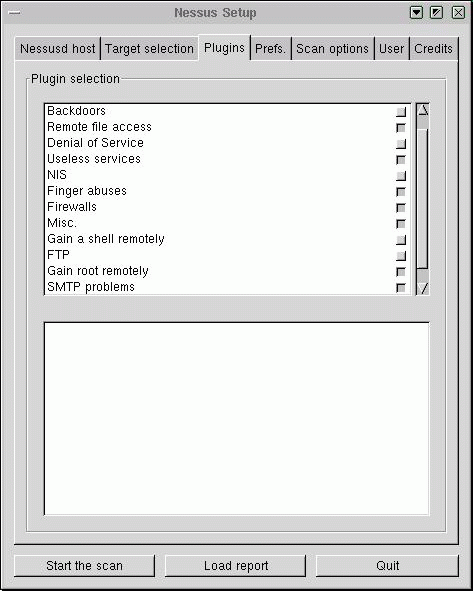
\includegraphics{nessus.png}
%\special{pdf:epdf (nessus.jpg)}
\caption{Interfaz gr\'afico de {\it Nessus}.}
\label{nessus}
\end{center}
\end{figure}
\\A pesar de la comodidad de estos interfaces gr\'aficos, muchos usuarios de 
Unix seguimos prefiriendo la potencia y flexibilidad de la l\'{\i}nea de
\'ordenes; {\it Nessus} tambi\'en ofrece la posibilidad de escanear un sistema
sin utilizar entorno gr\'afico, volcando los resultados en un archivo de 
texto:
\begin{quote}
\begin{verbatim}
luisa:~$ cat entrada
rosita
luisa:~$ nessus -q localhost 3001 toni entrada salida.rosita
Pass phrase: 
luisa:~$
\end{verbatim}
\end{quote}
La orden anterior conecta al servidor {\tt nessusd} situado en el puerto 3001
de la m\'aquina {\tt luisa} bajo el nombre de usuario {\tt toni}, y desde 
ah\'{\i} lanza un ataque a los sistemas indicados en el archivo {\tt entrada}
(en este caso, s\'olamente a {\tt rosita}); los resultados de dicho ataque se
depositan tras el escaneo en el archivo {\tt salida.rosita}, un fichero de 
texto normal y corriente:
\begin{quote}
\begin{verbatim}
luisa:~$ head -13 salida.rosita
rosita chargen (19/tcp)
rosita ftp (21/tcp)
rosita telnet (23/tcp) INFO The Telnet service is running. This service is 
dangerous in the sense that it is not ciphered - that is, everyone can sniff
the data that passes between the telnet client and the telnet server. This 
includes logins and passwords.
You should disable this service and use ssh instead.
Solution : Comment out the 'telnet' line in /etc/inetd.conf.
Risk factor : Low
rosita smtp (25/tcp)
rosita finger (79/tcp)
rosita www (80/tcp)
rosita sunrpc (111/tcp)
luisa:~$
\end{verbatim}
\end{quote}
\section{Crack}
{\it Crack}, desarrollado por el experto en seguridad Alec Muffet, es el
`adivinador' de contrase\~nas m\'as utilizado en entornos Unix; actualmente
se encuentra en su versi\'on 5\footnote{Aunque {\it Crack6} y {\it Crack7}
existen, no son realmente nuevas versiones del programa, sino un
rompecontrase\~nas minimalista y uno de fuerza bruta, respectivamente.}, que
funciona correctamente en la mayor\'{\i}a de clones del sistema operativo 
(Linux, Solaris, OSF\ldots). Ejecutar peri\'odicamente {\it Crack} sobre el
fichero de contrase\~nas de sus sistemas es algo {\bf muy recomendable} para
cualquier administrador m\'{\i}nimamente preocupado por la seguridad, sin
importar que se utilicen mecanismos para obligar a los usuarios a elegir
{\it passwords} aceptables.\\
\\Este adivinador realiza una primera pasada sobre el fichero de claves 
intentando romper contrase\~nas en base a la informaci\'on de cada usuario
almacenada en el archivo; se trata de unas comprobaciones r\'apidas pero
efectivas, ya que aunque la cantidad de datos del fichero no es muy grande, se
trata de informaci\'on frecuentemente utilizada como {\it password}. Tras
esta pasada, entran en juego los diccionarios para seguir adivinando 
contrase\~nas (un diccionario no es m\'as que un fichero con posibles {\it
passwords} en \'el, generalmente uno por l\'{\i}nea). El propio programa se 
distribuye con algunos de estos ficheros, pero es recomendable que se
complementen con m\'as diccionarios (existen multitud de ellos disponibles a
trav\'es de Internet), especialmente con aquellos que contengan palabras
que por las caracter\'{\i}sticas del sistema sean susceptibles de ser usadas
como claves; por ejemplo, si estamos en Espa\~na seguramente nos convendr\'a
utilizar un diccionario con palabras en castellano; si administramos una 
m\'aquina de un departamento de biolog\'{\i}a, otro con t\'erminos de esta
ciencia\ldots incluso si sospechamos que nuestros usuarios son aficionados al
deporte, o a la literatura griega antigua, podemos encontrar diccionarios
adecuados a estos campos.\\
\\Con todos estos diccionarios -- los propios y los que cada administrador puede
a\~nadir -- {\it Crack} construye una base de datos con la que empieza a 
trabajar; la primera pasada utilizando diccionarios consiste simplemente en
probar palabras con todas las letras en min\'usculas. Posteriormente, se
mezclan may\'usculas y min\'usculas, y de esta forma se van combinando 
caracteres hasta a\~nadir n\'umeros y caracteres alfanum\'ericos a cada palabra
de los diccionarios para comprobar que dicha combinaci\'on no es utilizada
como contrase\~na en el sistema. Habitualmente las primeras pasadas son las
que m\'as claves son capaces de romper, pero una vez adivinados los {\it
passwords} m\'as d\'ebiles quiz\'as nos interese seguir ejecutando {\it Crack}
para obtener contrase\~nas m\'as elaboradas: recordemos que un atacante
puede aprovechar la potencia de servidores en los que ha penetrado para ejecutar
{\it Crack} sobre nuestro fichero de contrase\~nas durante mucho tiempo, por lo
que es posible que `adivine' claves que {\it a priori} no son d\'ebiles.\\
\\Tal y como se explica en su documentaci\'on, la forma en que {\it Crack}
trata de adivinar contrase\~nas es seguramente la que consigue mayor velocidad;
en primer lugar se ordenan y se agrupan las entradas del fichero de {\it 
passwords} en base a su {\it salt} (ya comentamos el mecanismo de cifrado a la
hora de hablar de autenticaci\'on de usuarios). Una vez clasificadas, para
cada grupo de {\it salts} diferente se selecciona una entrada de diccionario
convenientemente tratada (may\'usculas, n\'umeros\ldots), se cifra utilizando
el {\it salt} (esto es lo que consume mayor tiempo de CPU) y se compara con
la contrase\~na cifrada de cada miembro del grupo; si coinciden, se ha
adivinado un nuevo {\it password}.\\
\\Para invocar a {\it Crack} utilizamos como argumento el fichero de claves a
atacar; por ejemplo, imaginemos que en lugar de nuestro {\tt /etc/passwd} vamos
a romper las contrase\~nas de otra de las m\'aquinas, guardadas en el fichero
{\tt `maquina'}:
\begin{quote}
\begin{verbatim}
luisa:/usr/local/c50a# ./Crack maquina
Crack 5.0a: The Password Cracker.
(c) Alec Muffett, 1991, 1992, 1993, 1994, 1995, 1996
System: Linux luisa 2.2.13 #6 Tue Apr 25 03:58:00 CEST 2000 i686 unknown
Home: /usr/local/c50a
Invoked: ./Crack maquina
Stamp: linux-2-unknown

Crack: making utilities in run/bin/linux-2-unknown
find . -name "*~" -print | xargs -n50 rm -f
( cd src; for dir in * ; do ( cd $dir ; make clean ) ; done )
make[1]: Entering directory `/usr/local/c50a/src/lib'
rm -f dawglib.o debug.o rules.o stringlib.o *~
make[1]: Leaving directory `/usr/local/c50a/src/lib'
make[1]: Entering directory `/usr/local/c50a/src/libdes'
/bin/rm -f *.o tags core rpw destest des speed libdes.a .nfs* *.old \
*.bak destest rpw des speed
make[1]: Leaving directory `/usr/local/c50a/src/libdes'
make[1]: Entering directory `/usr/local/c50a/src/util'
rm -f *.o *~
make[1]: Leaving directory `/usr/local/c50a/src/util'
make[1]: Entering directory `/usr/local/c50a/src/lib'
make[1]: `../../run/bin/linux-2-unknown/libc5.a' is up to date.
make[1]: Leaving directory `/usr/local/c50a/src/lib'
make[1]: Entering directory `/usr/local/c50a/src/util'
all made in util
make[1]: Leaving directory `/usr/local/c50a/src/util'
Crack: The dictionaries seem up to date...
Crack: Sorting out and merging feedback, please be patient...
Crack: Merging password files...
Crack: Creating gecos-derived dictionaries
mkgecosd: making non-permuted words dictionary
mkgecosd: making permuted words dictionary
Crack: launching: cracker -kill run/Kluisa.11110   
Done
luisa:/usr/local/c50a# 
\end{verbatim}
\end{quote}
Tras devolver el control al {\it shell} el adivinador estar\'a trabajando en
segundo plano:
\begin{quote}
\begin{verbatim}
luisa:/usr/local/c50a# ps   
  PID TTY          TIME CMD
10809 ttyp3    00:00:00 bash
11327 ttyp3    00:00:07 cracker
11330 ttyp3    00:00:00 kickdict <defunct>
11333 ttyp3    00:00:00 ps
luisa:/usr/local/c50a# 
\end{verbatim}
\end{quote}
Podemos comprobar el estado del ataque en todo momento utilizando la utilidad
{\tt Reporter}:
\begin{quote}
\begin{verbatim}
luisa:/usr/local/c50a# ./Reporter
---- passwords cracked as of Thu May  4 08:05:35 CEST 2000 ----

Guessed josel [beatriz]  Jose Luis,,0, [maquina /bin/ksh]

---- done ----
luisa:/usr/local/c50a# 
\end{verbatim}
\end{quote}
Y para finalizar la ejecuci\'on del adivinador utilizaremos el {\it shellscript}
{\tt plaster}:
\begin{quote}
\begin{verbatim}
luisa:/usr/local/c50a# ./scripts/plaster 
+ kill -TERM 11327
+ rm -f run/Kluisa.11110
+ exit 0
luisa:/usr/local/c50a# 
\end{verbatim}
\end{quote}
Para finalizar el punto, hay que volver a insistir sobre el uso regular de
{\it Crack} en cada una de las m\'aquinas bajo nuestra responsabilidad; aunque
muchos administradores consideran el utilizar este tipo de programas equipararse
a un pirata, hemos de pensar siempre que es mejor que las contrase\~nas 
d\'ebiles las encuentre el {\tt root} antes que un atacante. Y si el 
administrador no utiliza un adivinador de este estilo, puede dar por seguro que
un pirata no dudar\'a en hacerlo.
